
Si tomamos como referencia la~\cref{fig:hexagonalDiagram}, el diagrama más extendido de una arquitectura hexagonal, en nuestro caso si intercambiamos ExternalSystemAdapter por nuestro Dispatcher de eventos e introducimos servicios de dominio entre el caso de uso y la Entidad tendremos nuestro esquema de alto nivel de nuestra arquitectura hexagonal en la~\cref{fig:CreateTaskHexagonalDiagram}. Como vemos no logra ser explicativo, ya que hay puertos de salida que se convierten en puertos de entrada como es el caso del Dispatcher, y cuando queremos quitar lógica de negocio del caso de uso mediante servicios de dominio que impidan el acceso directo a los repositorios de persistencia dicho diagrama se va quedando pequeño. Es perferible diagramas UML tal y comose muestra en~\cref{fig:createTaskUseCaseArchitecture}

\begin{figure}[H]
    \centering
    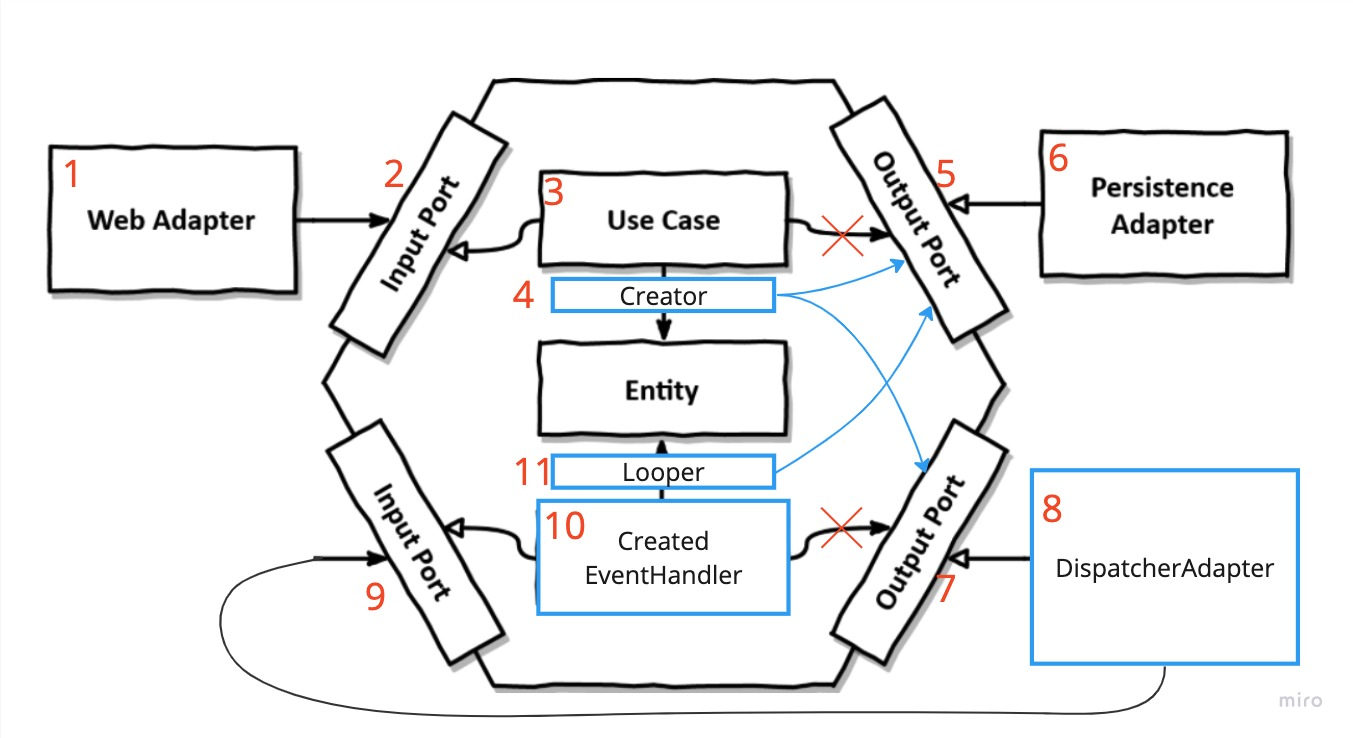
\includegraphics[height=0.3\textheight]{./part/Ejecucion/Seguimiento/CreateTaskUseCase/img/CreateTaskHexagonalDiagram}
    \caption{Hexagonal architecture diagram}\label{fig:CreateTaskHexagonalDiagram}
\end{figure}

\begin{figure}[H]
    \centering
    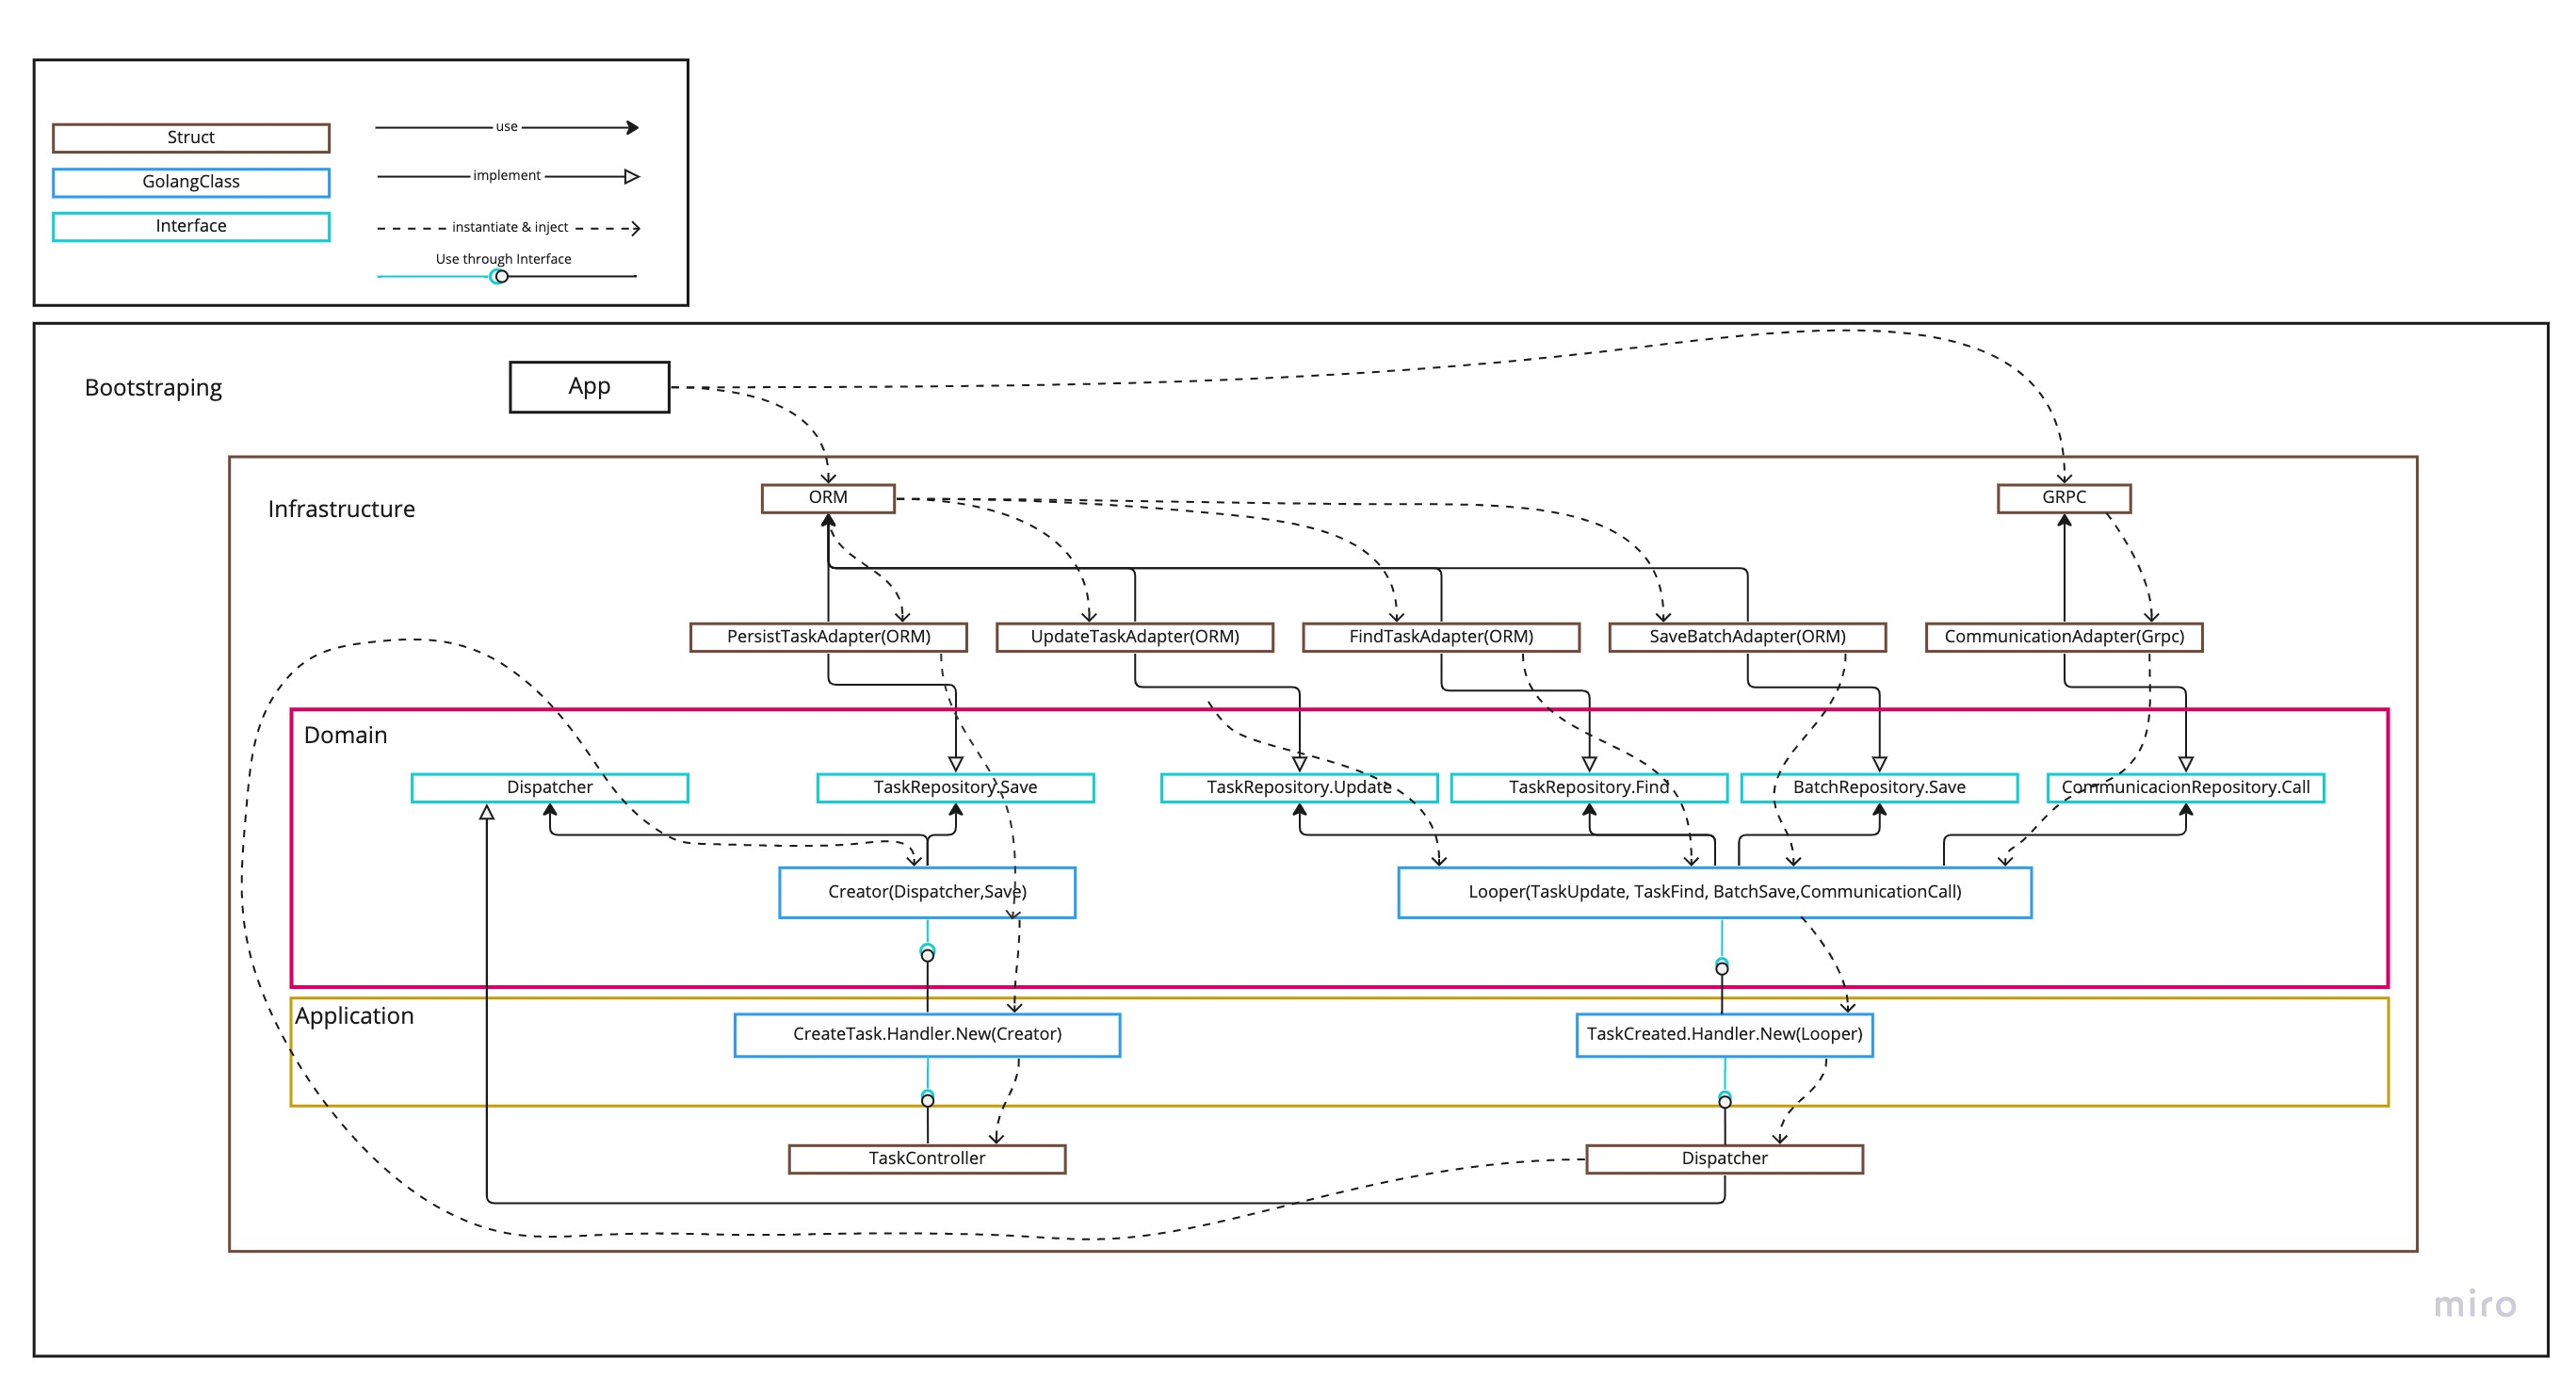
\includegraphics[height=0.3\textheight]{./part/Ejecucion/Seguimiento/CreateTaskUseCase/img/createTaskUseCaseArchitecture}
    \caption{CreateTaskUseCase hexagonal architecture diagram}\label{fig:createTaskUseCaseArchitecture}
\end{figure}

En el diagrama~\cref{fig:createTaskUseCaseArchitectureFolderStructure} podemos apreciar la interacción de componentes atendiendo a su distribución en nuestro diseño organizativo del código en ficheros.

\begin{figure}[H]
    \centering
    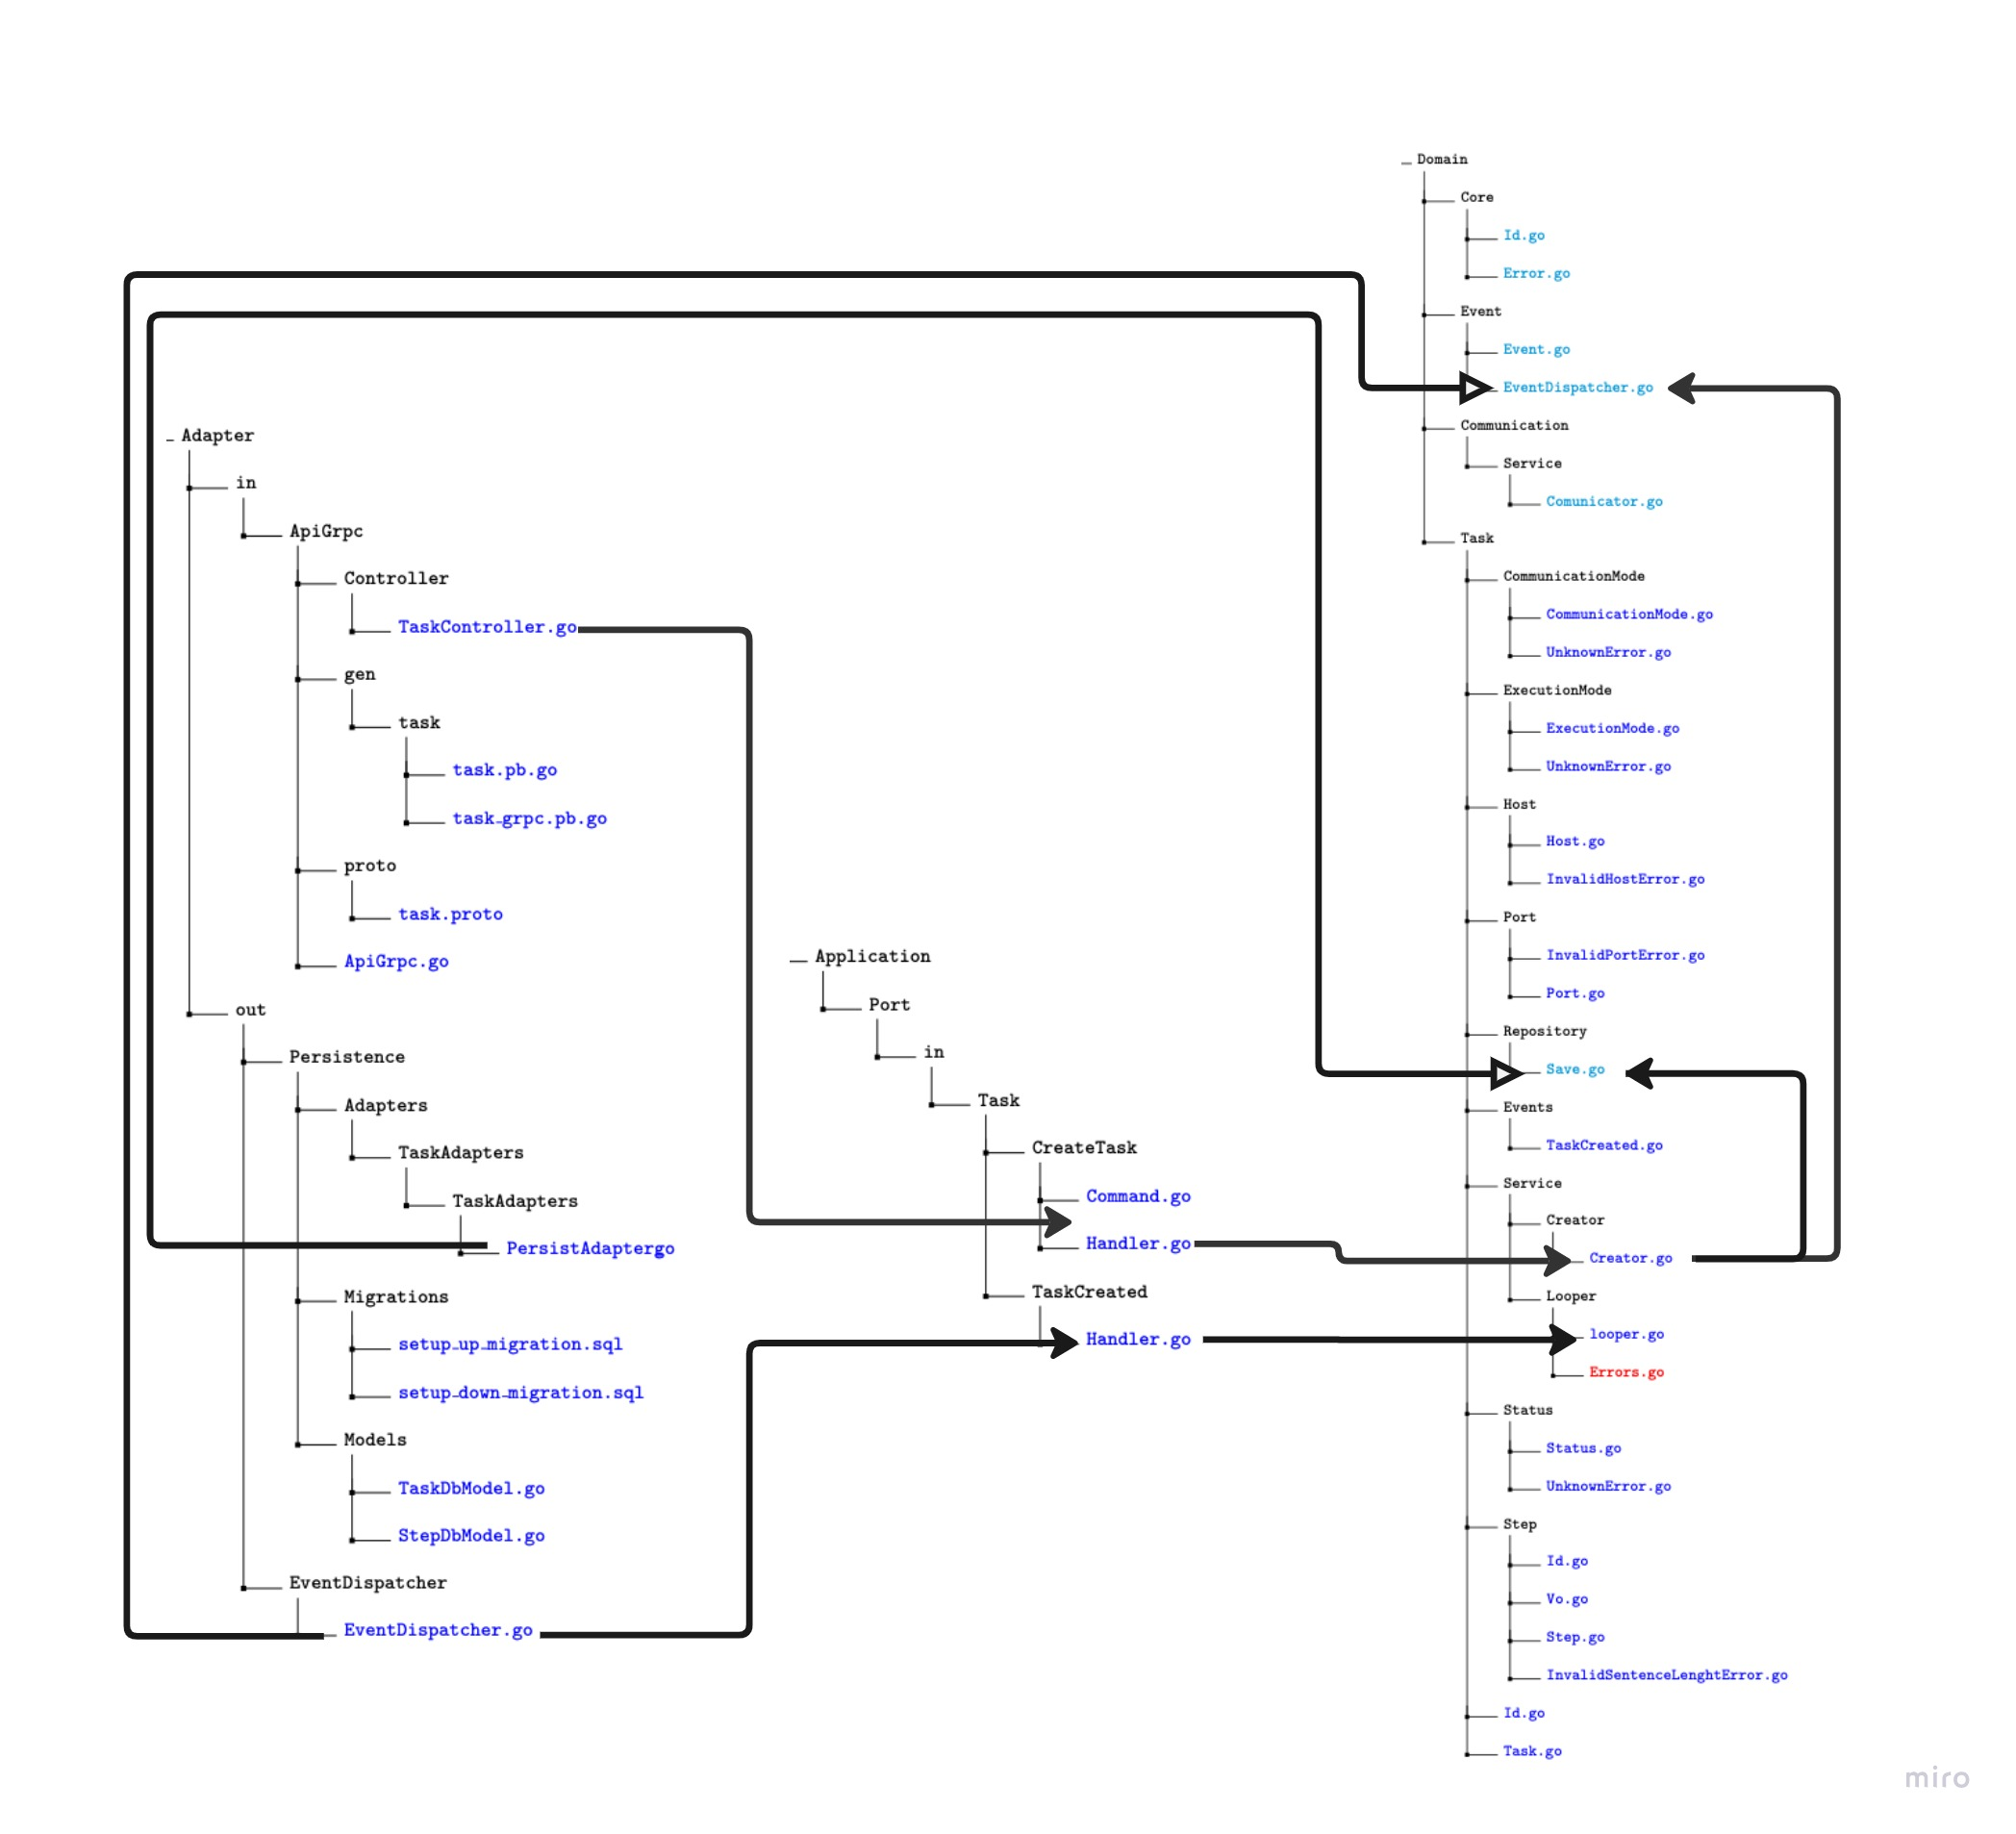
\includegraphics[height=0.5\textheight]{./part/Ejecucion/Seguimiento/CreateTaskUseCase/img/PFM - CreateUseCaseFolderStructure}
    \caption{CreateTaskUseCase folder Structure}\label{fig:createTaskUseCaseArchitectureFolderStructure}
\end{figure}

Con respecto a la estrategia de mapping Golang casi obliga al uso general de interfaces entre todos los elementos. Al necesitar el equivalente de la implementación de clase para garantizar la cohesión ya estamos utilizando interfaces para todas las clases. Así que en este caso utilizamos un fullMapping adaptado. De cara a decidir extraemos la recomendacion de~\cite{TomHombergs2019GYHD}:“
we might start with a simple strategy that allows us to quickly evolve the code and later move to a more complex one that helps us to better decouple the layers. In order to decide which strategy to use when, we need to agree upon a set of guidelines within the team. These guidelines should answer the question which mapping strategy should be the first choice in which situation. They should also answer why they are first choice so that we’re able to evaluate if those reasons still apply after some time.“

Al final se trata de tomar una decisión en equipo, documentar las razones y ser consistentes. Reevaluar las razones ante un reto que las ponga a prueba y tomar o no la decisión de cambiar la estrategia. Dentro de la estrategia fullmapping se debe implementar un modelo tanto de entrada, como ya se contempla, como de salída. Es decir, la respuesta que hay entre cada capa también debe ser mappeada, podemos ver el patrón readaptado en la figura~\cref{fig:GetHandMapping}

\begin{figure}[H]
    \centering
    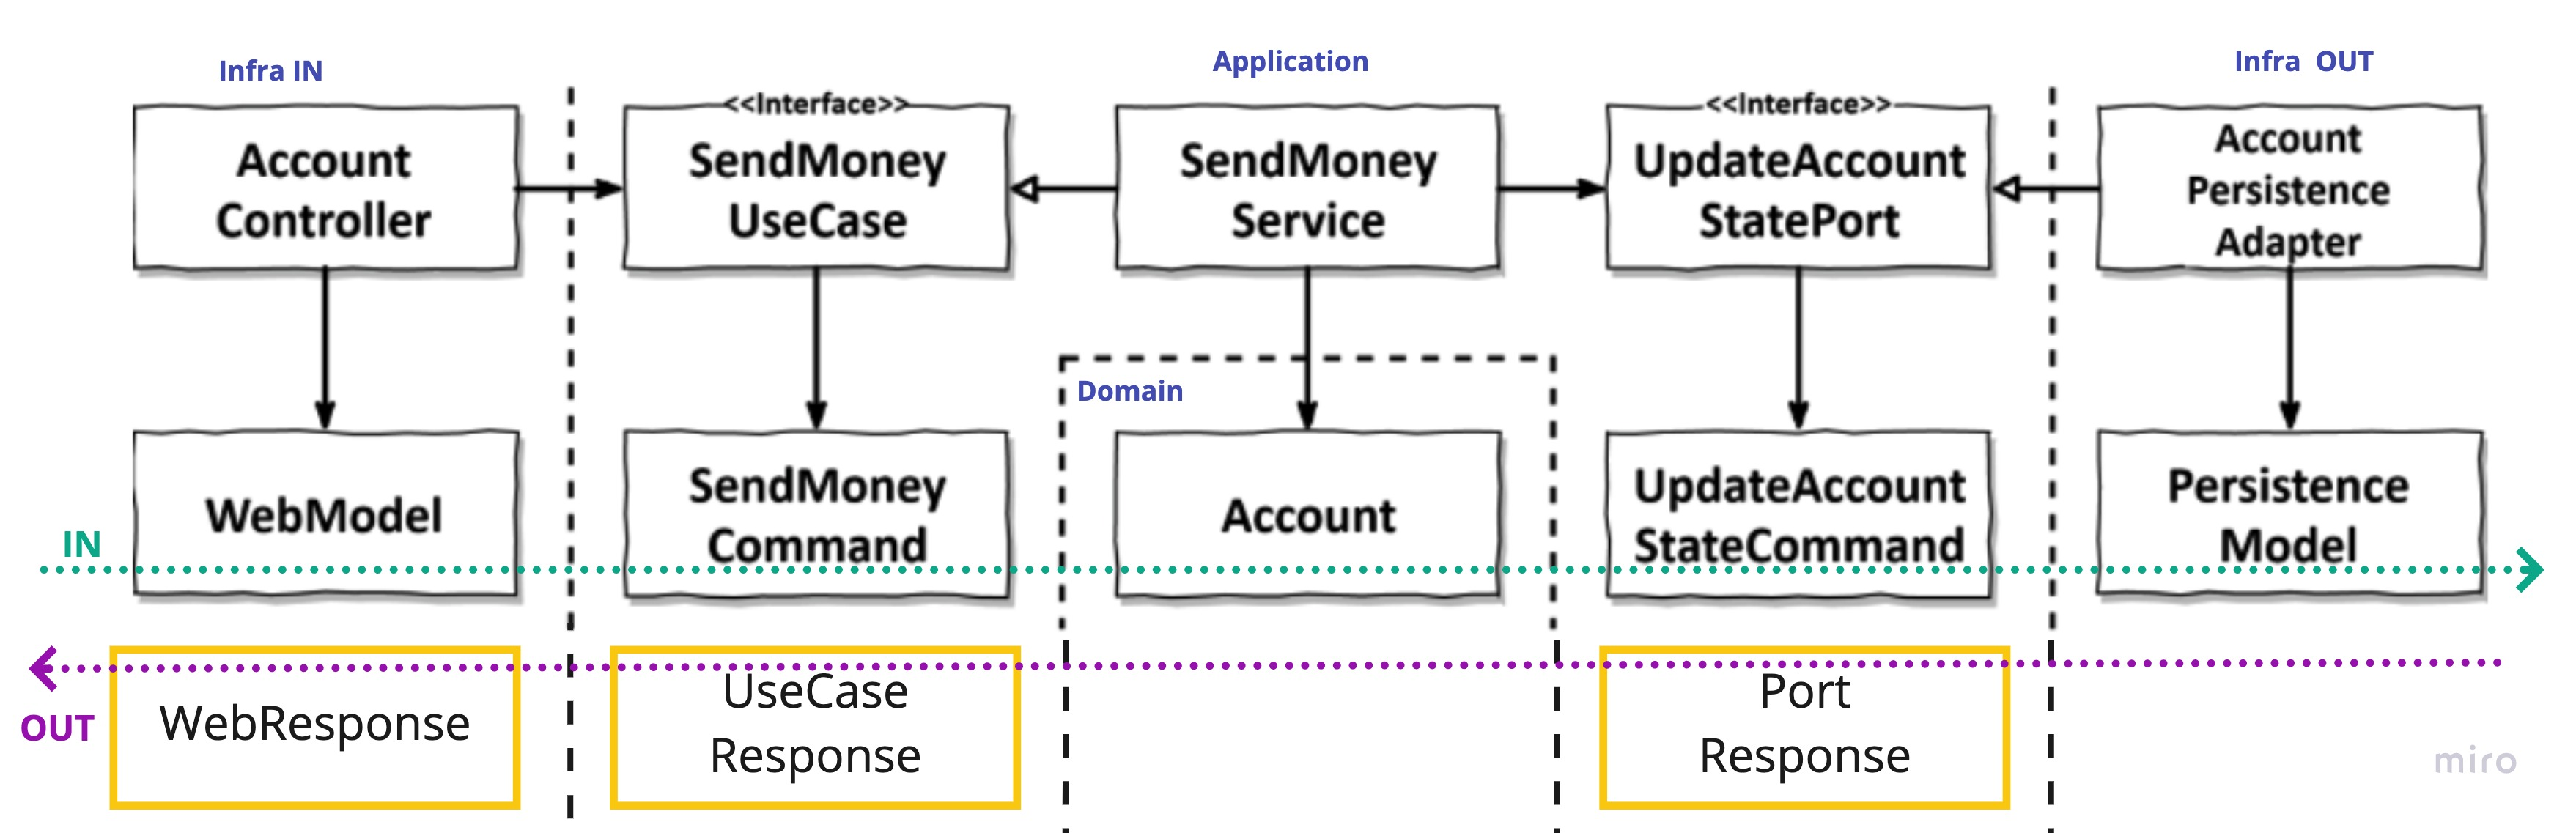
\includegraphics[height=0.2\textheight]{./part/Ejecucion/Seguimiento/CreateTaskUseCase/img/PFM - GetHandMapping}
    \caption{CreateTaskUseCase folder Structure\cite{TomHombergs2019GYHD}}\label{fig:GetHandMapping}
\end{figure}

Claramente esto aumenta la burocracia y finalmente la opción que hemos tomado se puede ver en la figura~\cref{fig:CreateTaskUseCaseMapping} En rojo se han marcado los atajos que se han tomado, es decir, el mapeo que no se ha implementado. El objetivo es aislarse bien de los puertos de entrada, es decir el GRPC, y no tanto de los puertos de salida. ya que la persistencia está bien aislada mediante las interfaces. Dentro de los adaptadores se hará el trabajo de mapeo entre las entidades de dominio y los modelos de persistencia y se traducirá de nuevo a dominio para responder.

\begin{figure}[H]
    \centering
    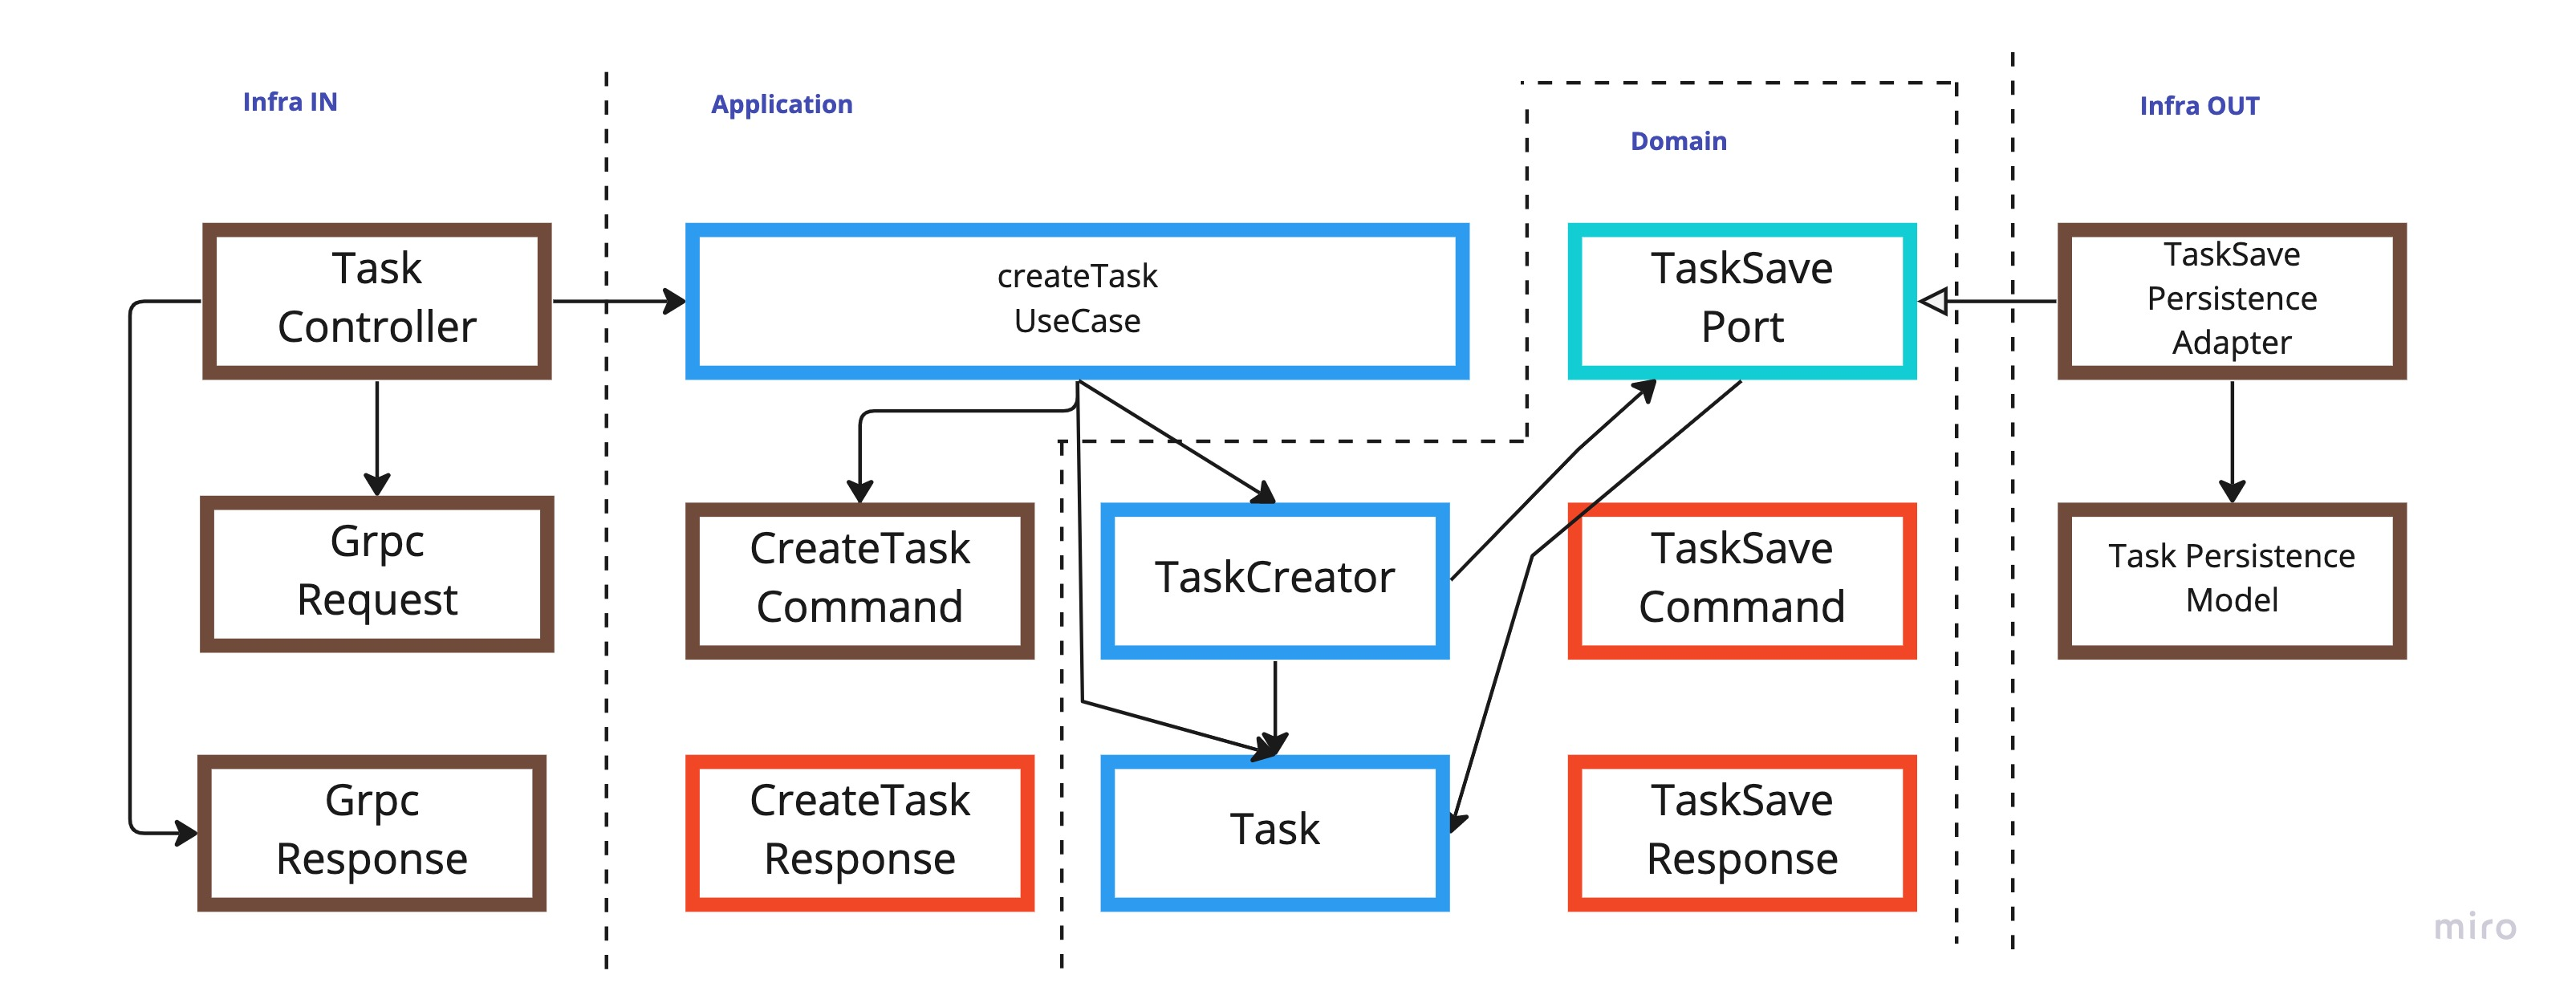
\includegraphics[height=0.2\textheight]{./part/Ejecucion/Seguimiento/CreateTaskUseCase/img/PFM - FinalMapping}
    \caption{CreateTaskUseCase folder Structure}\label{fig:CreateTaskUseCaseMapping}
\end{figure}

Ahora vamos a exponer el código final de este caso de uso, vamos a hacer referencia a:
\begin{itemize}
    \item TaskController~\cref{fig:TaskControler}
    \item CreateTaskUseCase~\cref{fig:CreateTaskUseCaseCode}
    \item Creator~\cref{fig:Creator}
    \item SavePort~\cref{fig:SavePort}
    \item PersistAdapter~\cref{fig:SaveAdapter}
    \item DispatcherPort~\cref{fig:DispatcherPort}
\end{itemize}

En el controller podemos ver como~\cref{fig:TaskControler} haciendo uso de la request entrante componemos el comando que corresponde y utilizando el usecase inyectado en el controller lo ejecutamos. El recuadro rojo de la imagen lo resalta. También es interesante resaltar que una vez ejecutado el caso de uso hacemos uso de la respuesta, que contiene el id de la nueva Task creada para devolverlo, pero tal y como vemos en el diagrama~\cref{fig:CreateTaskUseCaseMapping} no hacemos uso directo de esta respuesta si no que componemos una nueva para el protocolo de comunicación que está utilizando el cliente, en este caso RPC

\begin{figure}[H]
    \centering
    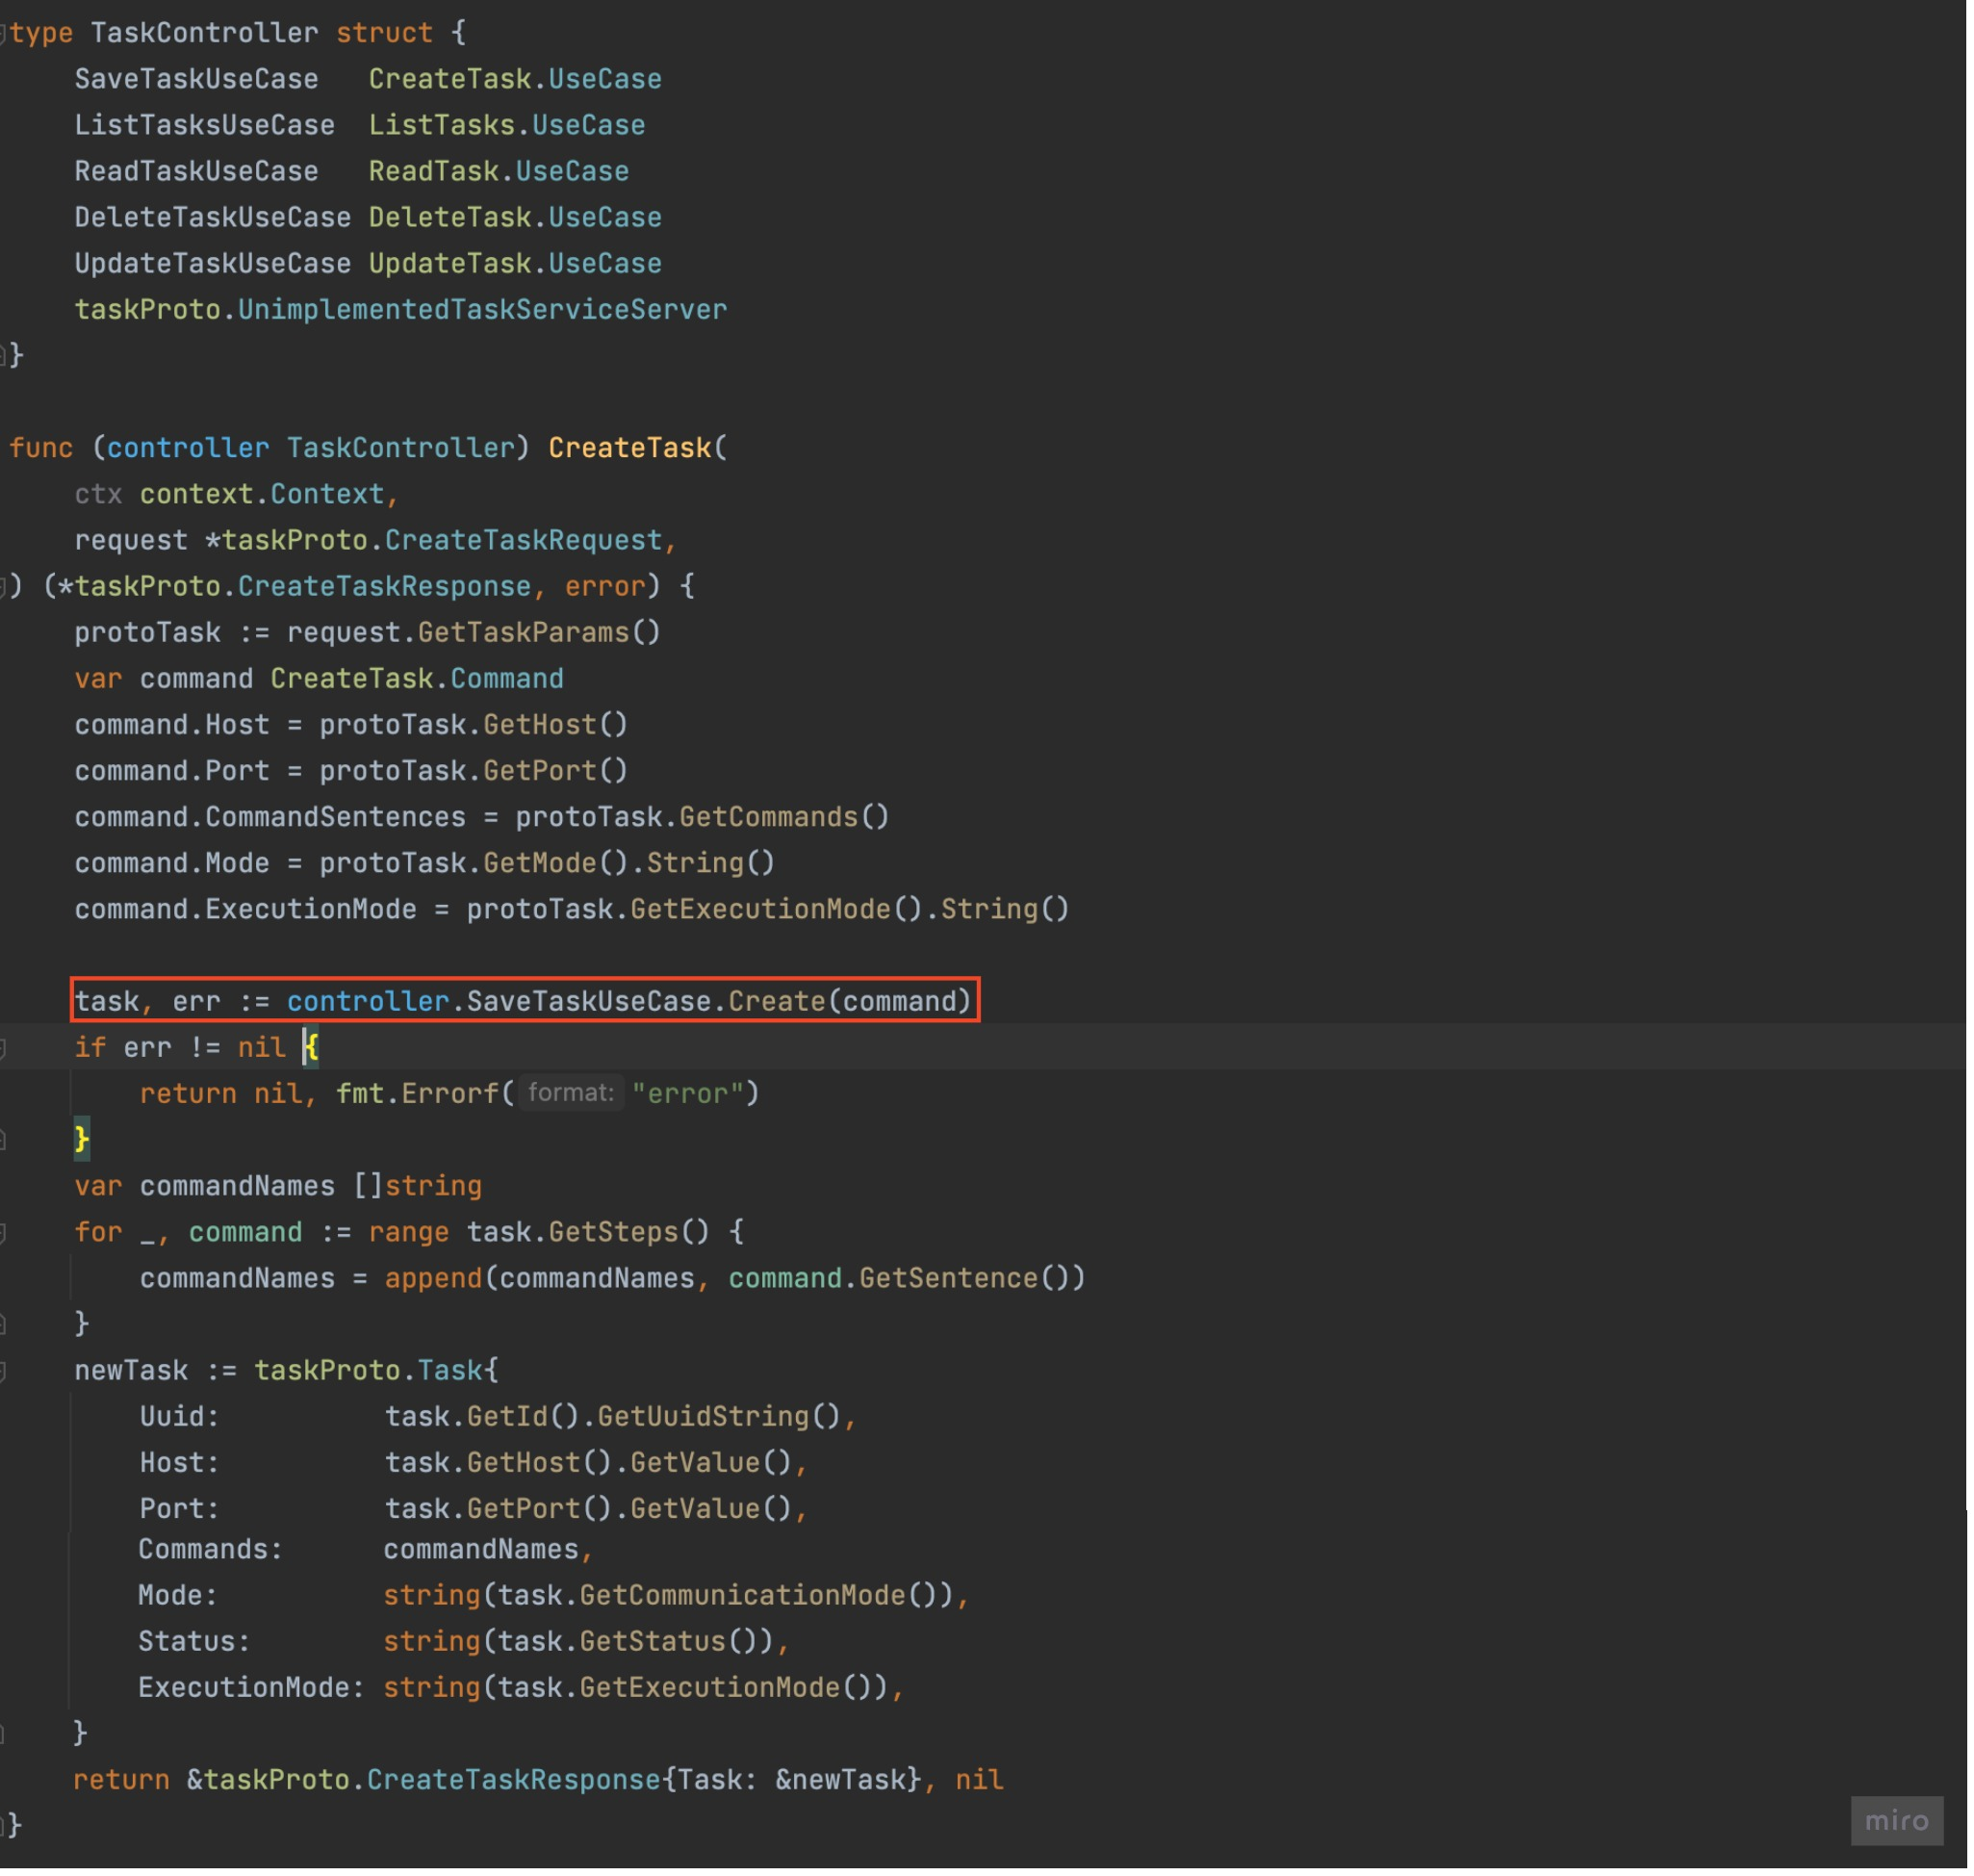
\includegraphics[height=0.5\textheight]{./part/Ejecucion/Seguimiento/CreateTaskUseCase/img/PFM - TaskController}
    \caption{TaskController.go}\label{fig:TaskControler}
\end{figure}

En el caso de uso que podemos ver en~\cref{fig:CreateTaskUseCaseCode} se resalta los imports, que suele ser un check rápido de que la arquitectura y los boundaries se están respetando. en este caso vemos que todo corresponde a Dominio. Siendo el caso de uso correspondiente a aplicación las dependencias van hacia adentro. También vemos que no tiene imports de librerías de terceros, es decir, infraestructura. Vemos que la interface UseCase está en mayúsculas exponiendola hacia afuera, mientras que el struct useCase está en minuscula no pudiendo ser utilizado fuera del package. Vemos que en el caso de uso se realiza la creación de los ValueObjects necesarios para la creación de una Task. Asegurando que no dan ningún error los datos de entrada y luego, haciendo uso del servicio se procede a crearla.

\begin{figure}[H]
    \centering
    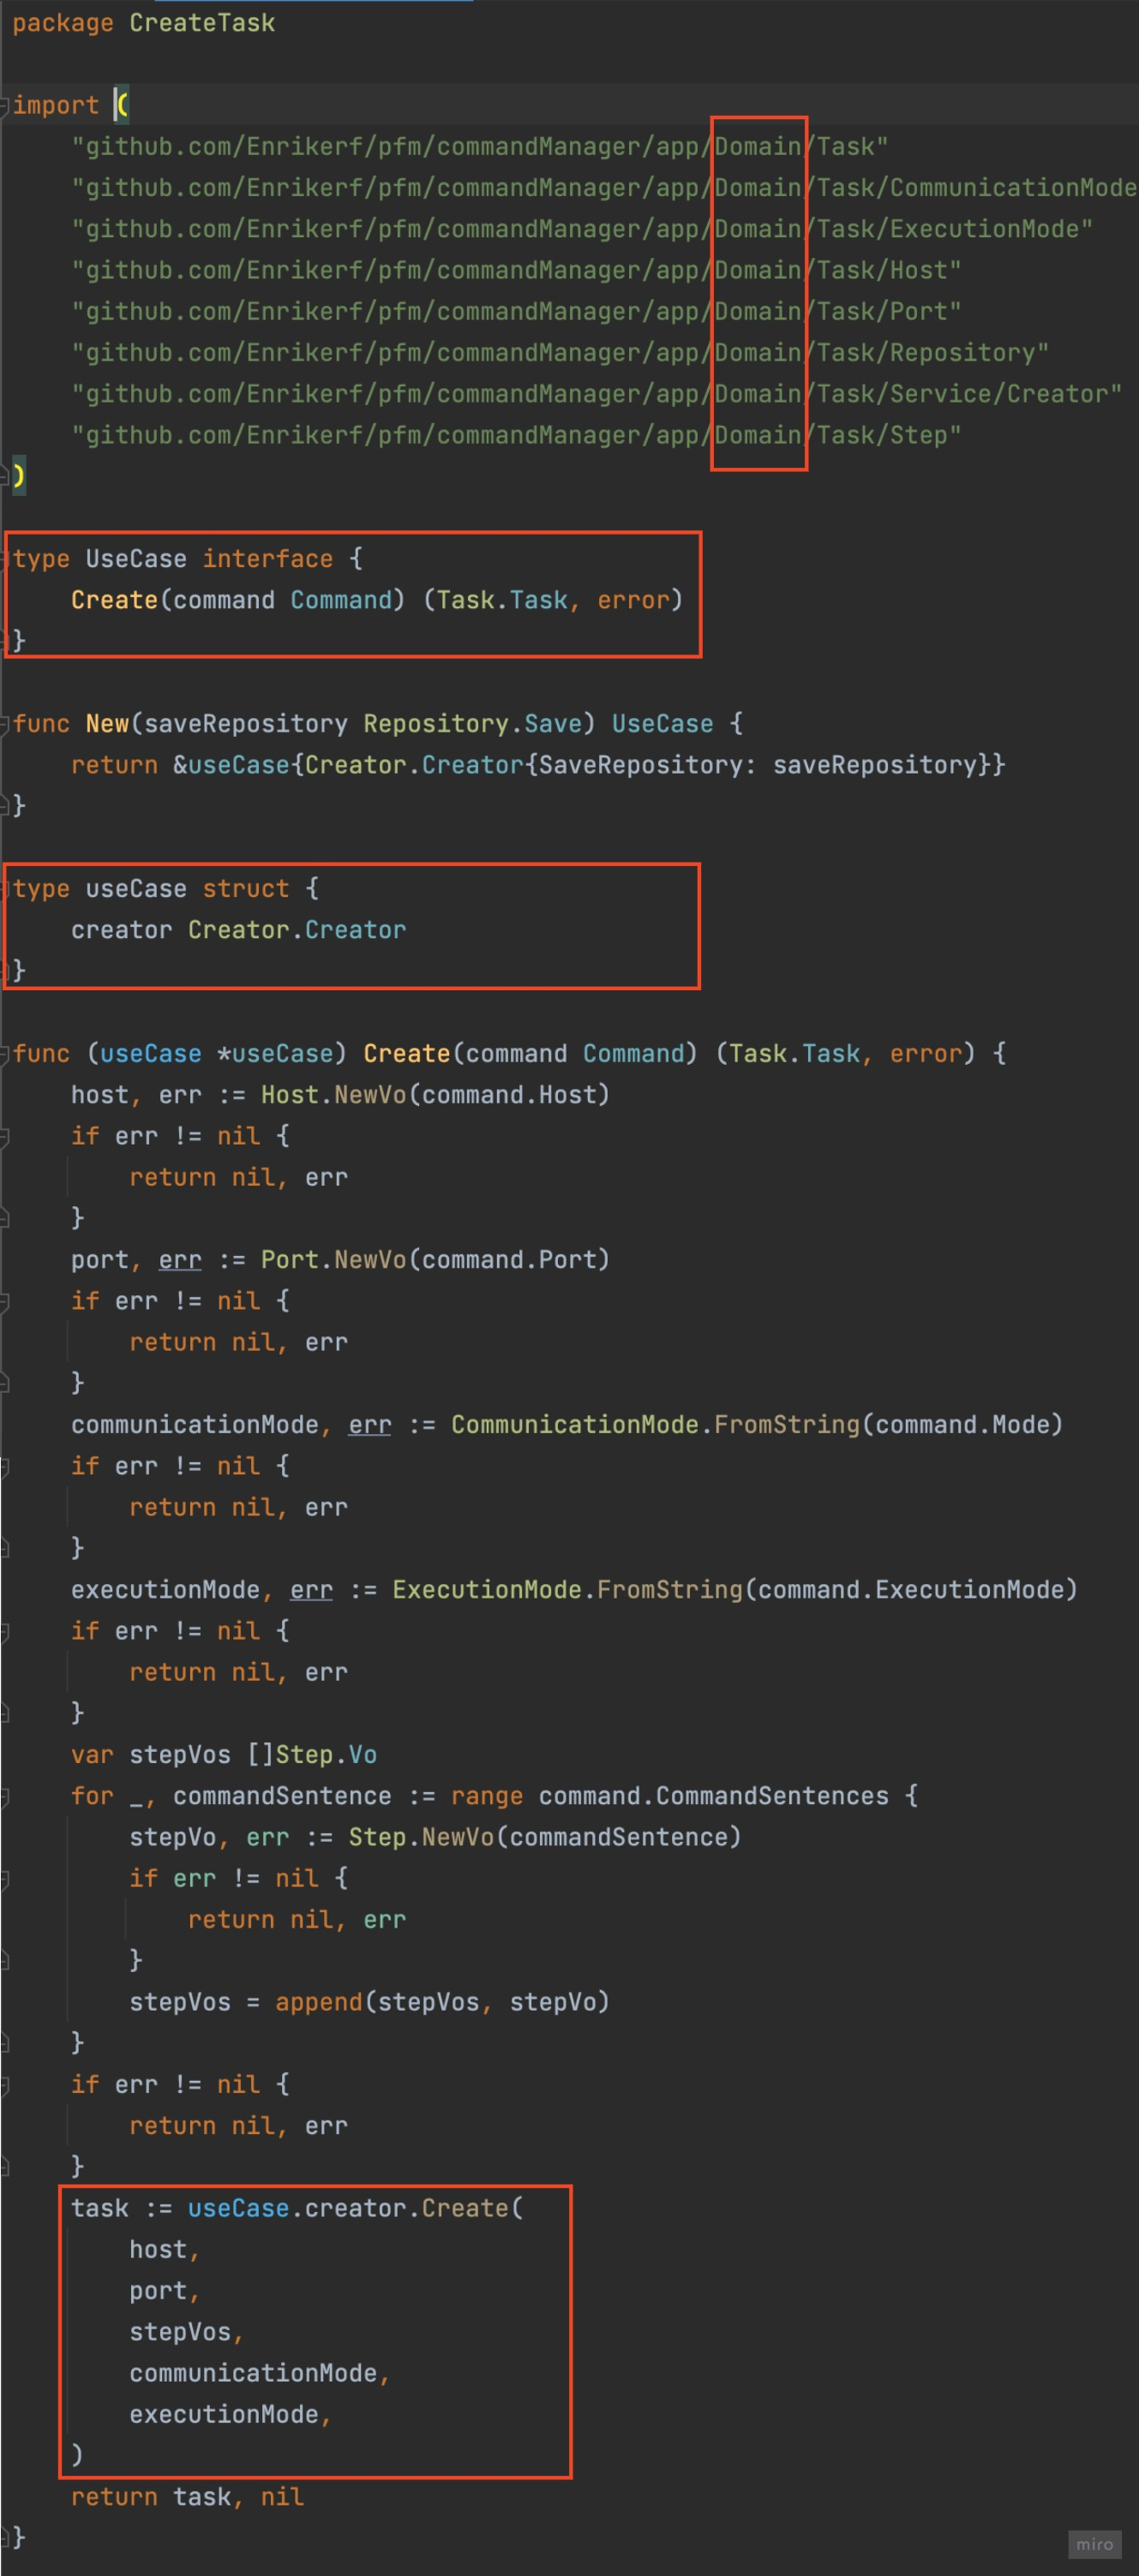
\includegraphics[height=0.5\textheight]{./part/Ejecucion/Seguimiento/CreateTaskUseCase/img/PFM - CreateTaskUseCaseCode}
    \caption{CreateTaskUseCaseCode.go}\label{fig:CreateTaskUseCaseCode}
\end{figure}

El servicio de Dominio Creator se encarga de encapsular y atomizar los procesos que tienen que ocurrir en bloque siempre que se desee crear una Task. Entre los cuales está instanciar la tarea con los ValueObjects que recibe como parámetros. Persistir la misma en la base de datos a través del puerto de salida, interfaz que implementará un adaptador. y emitir el evento de creación a través del otro puerto de salida, el Dispatcher interfaz que implementará otro adaptador. En la sección de \textit{imports} se aprecia que no hay elementos de infraestructura o aplicación. Se limita al uso de Dominio. Aislados del exterior.

\begin{figure}[H]
    \centering
    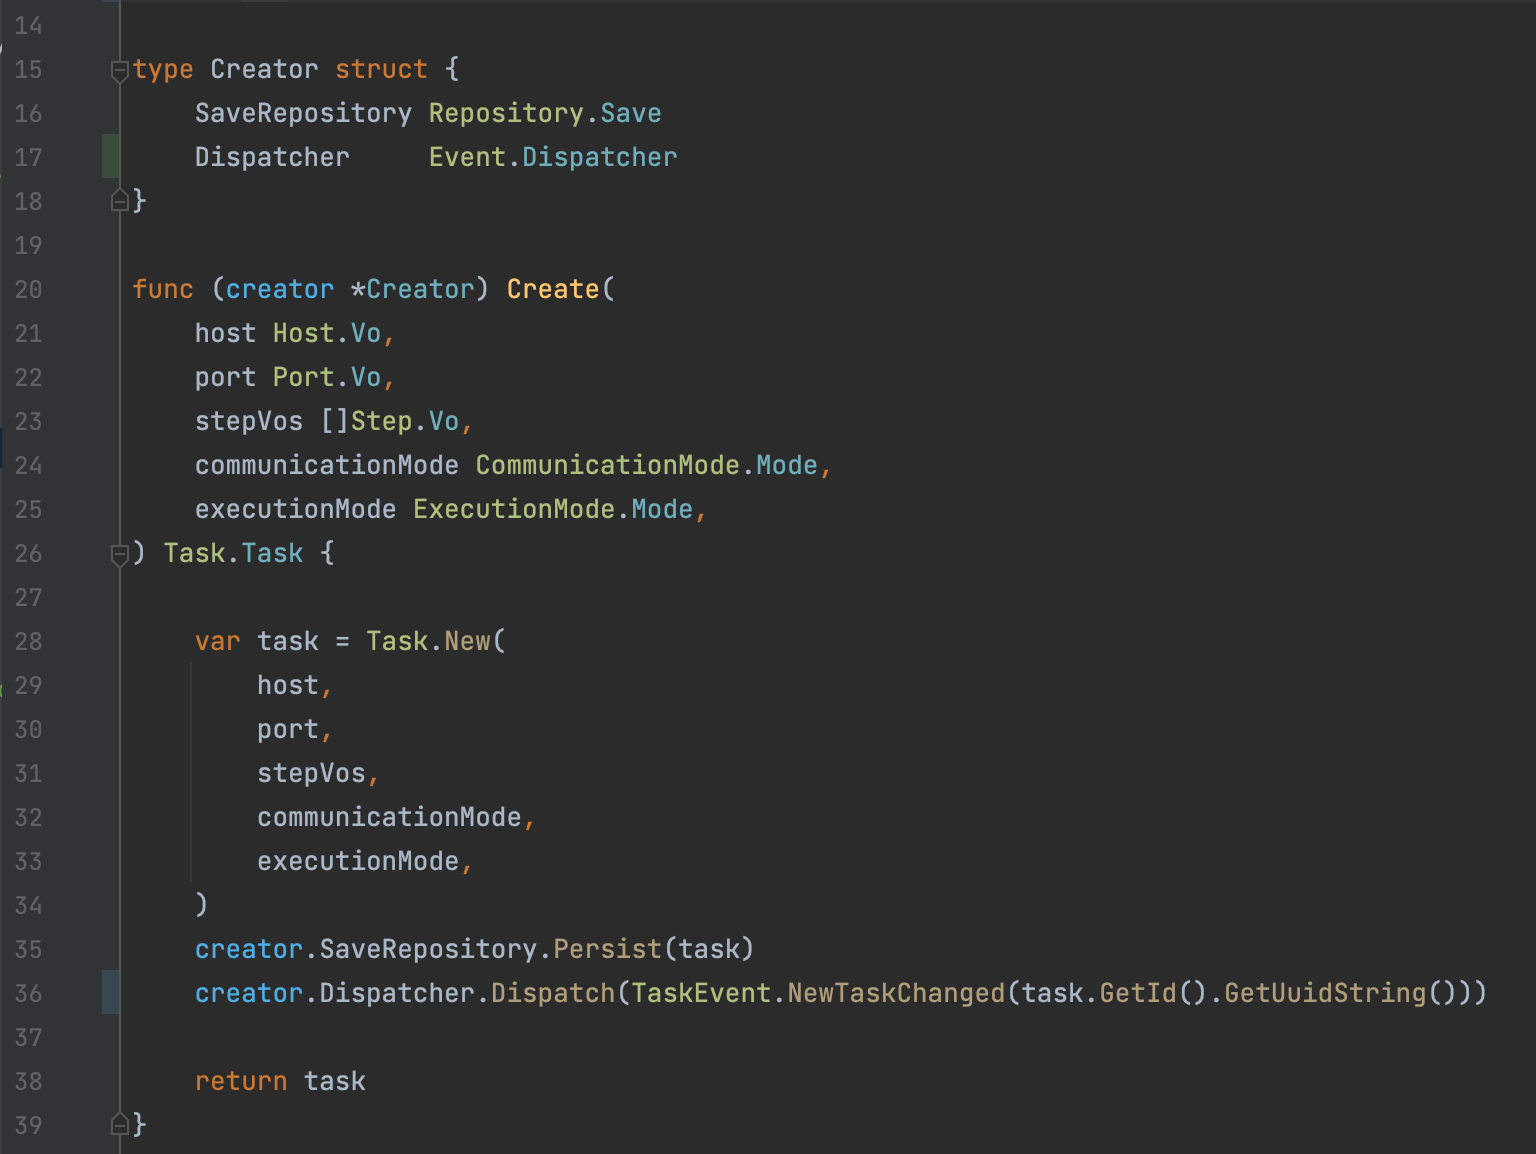
\includegraphics[height=0.4\textheight]{./part/Ejecucion/Seguimiento/CreateTaskUseCase/img/PFM - creator}
    \caption{Creator.go}\label{fig:Creator}
\end{figure}

\begin{figure}[H]
    \centering
    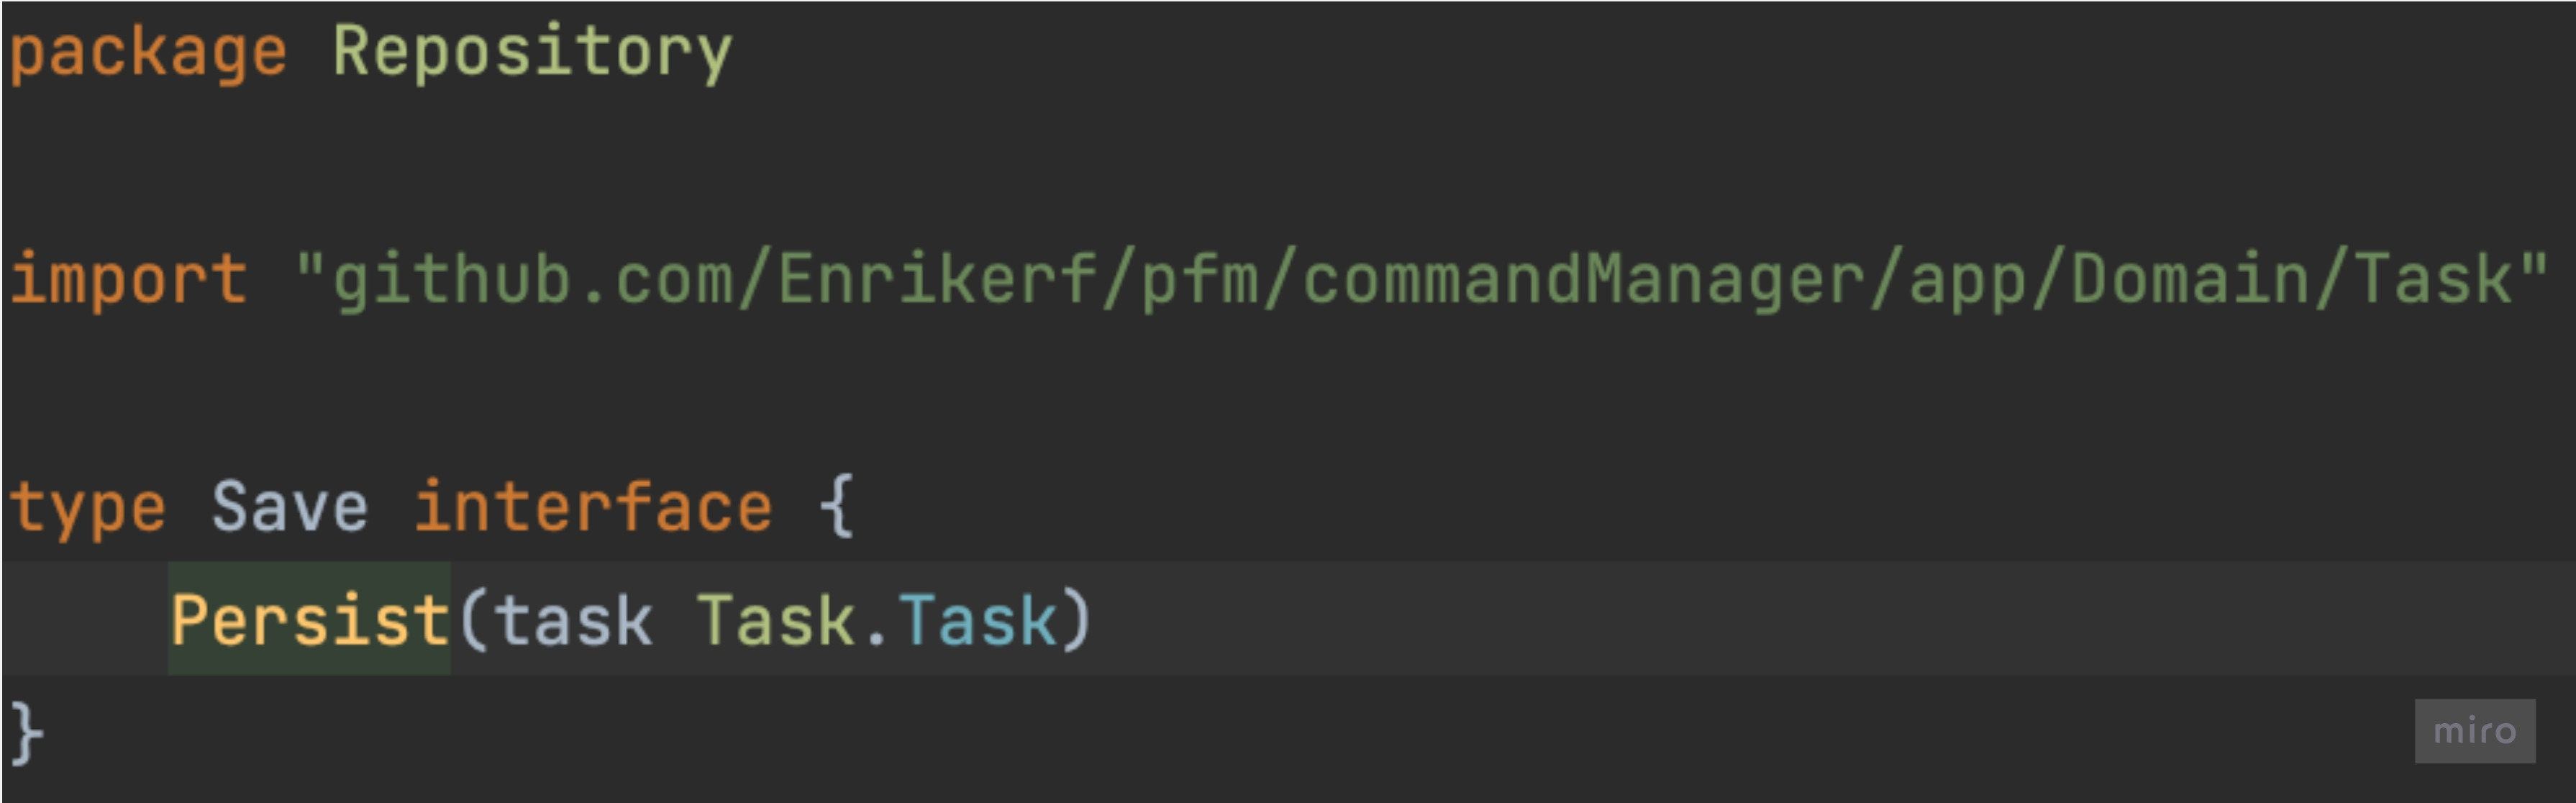
\includegraphics[height=0.2\textheight]{./part/Ejecucion/Seguimiento/CreateTaskUseCase/img/PFM - SavePort}
    \caption{SavePort.go}\label{fig:SavePort}
\end{figure}

\begin{figure}[H]
    \centering
    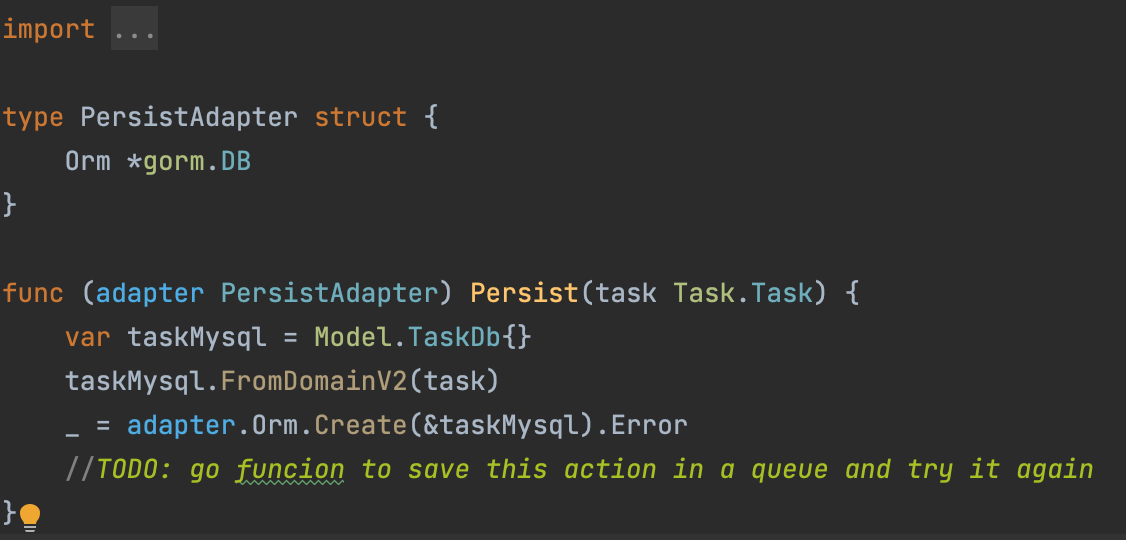
\includegraphics[height=0.25\textheight]{./part/Ejecucion/Seguimiento/CreateTaskUseCase/img/PFM - SaveAdapter}
    \caption{SaveAdapter.go}\label{fig:SaveAdapter}
\end{figure}

\begin{figure}[H]
    \centering
    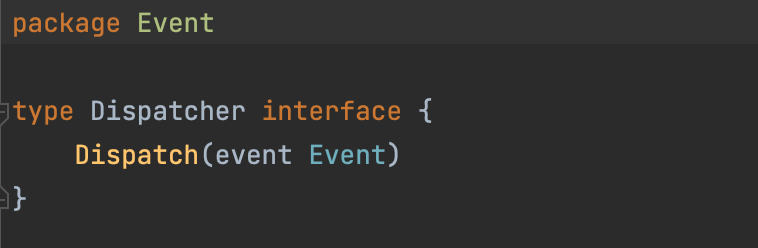
\includegraphics[height=0.15\textheight]{./part/Ejecucion/Seguimiento/CreateTaskUseCase/img/PFM - Dispatcher}
    \caption{Dispatcher.go}\label{fig:DispatcherPort}
\end{figure}